\documentclass[12pt, oneside]{article}   	% use "amsart" instead of "article" for AMSLaTeX format
\usepackage{textcomp}
\usepackage{geometry}                		% See geometry.pdf to learn the layout options. There are lots.
\geometry{letterpaper}                   		% ... or a4paper or a5paper or ... 
%\geometry{landscape}                		% Activate for rotated page geometry
%\usepackage[parfill]{parskip}    		% Activate to begin paragraphs with an empty line rather than an indent
\usepackage{graphicx}				% Use pdf, png, jpg, or eps§ with pdflatex; use eps in DVI mode
\usepackage{caption}
\usepackage{subcaption}								% TeX will automatically convert eps --> pdf in pdflatex		
\usepackage{color}
\usepackage{amssymb}
\usepackage{amsthm}
\usepackage{url}
\newtheorem{theorem}{Theorem}
\newtheorem{definition}{Definition}
\usepackage{natbib}
\usepackage{xcolor}
% removed hyperref because of arXiv complaining
\usepackage{authblk}
\usepackage{float}
\usepackage{rotating}
\usepackage{adjustbox}
\usepackage[font=small,labelfont=bf]{caption}
%\usepackage{changes}
\usepackage{changes}
\definechangesauthor[name={George Chacko}, color=blue]{gc}

\usepackage{authblk}
\title{Finding Well-Connected Communities in Real-World Networks}
\author[1]{Minhyuk Park\thanks{author order to be determined later}}
\author[1]{Yasamin Tabatabaee\thanks{author order to be determined later}}
\author[1]{Baqiao Liu\thanks{author order to be determined later}}
\author[1]{Placeholder1\thanks{author order to be determined later}}
\author[1]{Placeholder2\thanks{author order to be determined later}}
\author[1]{Placeholder3\thanks{author order to be determined later}}
\author[2]{Dmitriy Korobskiy}
\author[1,3]{George Chacko\thanks{chackoge@illinois.edu}}
\author[1]{Tandy Warnow\thanks{warnow@illinois.edu}}
\affil[1]{Department of Computer Science, University of Illinois Urbana-Champaign, Urbana, IL 61801}
\affil[2]{NTT DATA, McLean, VA 22102}
\affil[3]{Office of Research, Grainger College of Engineering, University of Illinois Urbana-Champaign, Urbana, IL 61801}

% \setlength{\parindent}{0pt}
%SetFonts

% ORCID IDs

% Baqiao Liu: 0000-0002-4210-8269
% Tandy Warnow: 0000-0001-7717-3514
% George Chacko: 0000-0002-2127-1892

\begin{document}
\maketitle
	
\abstract{Community detection in real-world networks is typically addressed through the use of graph clustering methods that partition the nodes of a 
network into disjoint subsets. While  the definition of community varies across methods, it is generally accepted that a elements of a community 
should be ``well-connected".  Applying a mild definition of well-connectedness, we explore features of clusters generated by the Leiden algorithm  and the Iterative K-core clustering algorithm. We evaluate 
clusters that are produced  by these two approaches for their susceptibility to become disconnected by the deletion of a small number of edges, and find that both methods produce some 
clusters that are poorly connected  when applied to real-world networks.  We use a modular pipeline to enable well-connected output clusters, in which allows a user specifies criteria 
for a valid  community considering cluster size and minimum edge cut size. We describe the use of this pipeline on real world networks and benchmark networks.
The differences we observe between real world and the synthetic networks are compelling: while clusters produced on real-world networks are often poorly connected, clusters computed 
on synthetic networks  generated by the LFR methodology, are more well-connected. A basic assumption of the LFR network generation process  is that every vertex  is in a community; therefore, this  study 
suggests the possibility that community structure is not globally found within real-world networks, and that clusterings should be further evaluated.}
	
\clearpage
	
\section{Introduction} 

The problem of finding communities in complex networks can be posed as a {\em graph partitioning} problem, where the input is a network (a graph with vertices and edges) and the
objective is a partitioning of the vertices into disjoint subsets, so that each of the subsets represents a community \citep{Girvan_2002,Newman_2004}. Community 
detection in  large networks has broad applications that include, in scientometrics, the detection of research areas, and author communities \citep{Waltman_2012,Li2014,Fiallos2017,Traag_2019,Chandrasekharan_2020,Wedell2022}.

Disjoint partition is a  common approach to community detection studies \citep{Fortunato2022,Fortunato2010} although variations on this theme arise from different scientific interests \citep{Coscia2011,Schaub2017}. 
A common feature of these different formulations is that  the elements of a community are more connected to each other than to those outside the community. In other words, a community 
should be {\em well-connected}. Using graph-theoretic terminology, a cluster is said to be well-connected if it does not have a small edge cut, which means that there should not be a small set of edges whose deletion 
disconnects the cluster; see discussion in \cite{Traag_2019}. 

While the concept of being well-connected depends on the size of the edge cut, the definition of what is ``too small" can be formulated in two
natural ways.
The first way
requires that an edge cut  $E_0$ be above some value derived from the number $n$ of 
vertices in the cluster $C$ such as $$||E_0|| \geq \log_{10}(||C||),$$    where $||.||$ denotes the number of elements in the given set.
Note that every edge in  a tree cluster is a cut edge, so a tree is  a compelling example of a poorly connected cluster. 
This formulation offers a relatively weak bound for large clusters (i.e., when   $n$ is large), but does provide some constraints on small clusters. 

A second approach, which is used in providing guarantees for the widely used Leiden algorithm \citep{Traag_2019}, evaluates the size of an edge cut by the split  of the cluster into two parts produced 
when the edge cut is removed from a cluster. Here it is required that the edge cut size be at least a fraction of the number of possible edges between the two  parts.
As proven, Equation D1 in the supplementary information in \cite{Traag_2019}, given any optimal CPM clustering of a network using resolution parameter $\gamma$, if an edge cut $E_0$
separates a cluster into two sets $A$ and $B$ then $$||E_0|| \geq \gamma ||A|| \times ||B||$$ This is a strong guarantee when the cluster is large,  but as it depends on the user-specified value for $\gamma$, it 
may have no guarantee  beyond being connected for small clusters. Thus, the two approaches provide guarantees about clusters being well-connected for different size clusters, with the first approach a stronger 
guarantee for small to moderate-sized clusters, and the second approach providing a stronger guarantee on the larger clusters.

To explore well connectedness in community detection, we performed a study to evaluate  clusters produced by two different clustering methods \citep{Traag_2019,Wedell2022}, the Leiden algorithm (Leiden) and Iterative K-core Clustering (IKC). We designed a pipeline to work with both Leiden and IKC that would ensure that all output clusters satisfy two constraints for being valid communities: (1) each cluster meets a minimum user-specified size requirement
and (2) each cluster is well-connected. For well-connectedness, we applied a mild criterion that for every cluster, the minimum edge-cut size must be greater than $\log_{10}n$, where $n$ is the number of vertices in the cluster. \textcolor{blue}{@tandy A reasonable question would be, ``Why did you pick the first of the two criteria to the exclusion of the second? Perhaps we want to say that Leiden already offers the second so we evaluated using the first?''}

The pipeline takes a Leiden or IKC clustering as input, and first removes all clusters that fail to meet a minimum size specified by the user or are trees. It then checks each remaining cluster for being well-connected; if a cluster fails this check so that it has a small edge cut, the minimum edge cut is deleted from the cluster, thus producing a set of subsets.  Each of these subsets are then re-clustered using the selected clustering method (IKC or Leiden), and the process recurses on the resultant set of clusters.

We find that for both Leiden and IKC, the pipeline results in reduced node coverage, defined in this study as the fraction of nodes in clusters that exceed the minimum user specified bound. The magnitude of this reduction is greater for Leiden than IKC, which can be explained in part by the fact that IKC clusters are k-cores. Further, the extent to which node coverage is reduced depends on the network being clustered. Beyond its use in understanding the nature of clusters generated by We either Leiden or IKC, the pipeline is likely to have practical use in providing additional guarantees of well connectedness that are specified by a user. 

\section{Materials and Methods}

\subsection{Methods} 
\emph{Pipeline Design} A modular pipeline was developed that (i) generated a clustering from an input network, (ii) filtered the resultant clusters to remove small clusters below size $B$ (where $B=11$ by default), and any trees, (iii) applied \emph{Connectivity Modifier} (CM), a recursive  method that modifies the clustering to ensure that all output clusters are well-connected, and (iv) remove any resultant small clusters.

\vspace{2 mm}

\begin{figure}[H]
\centering
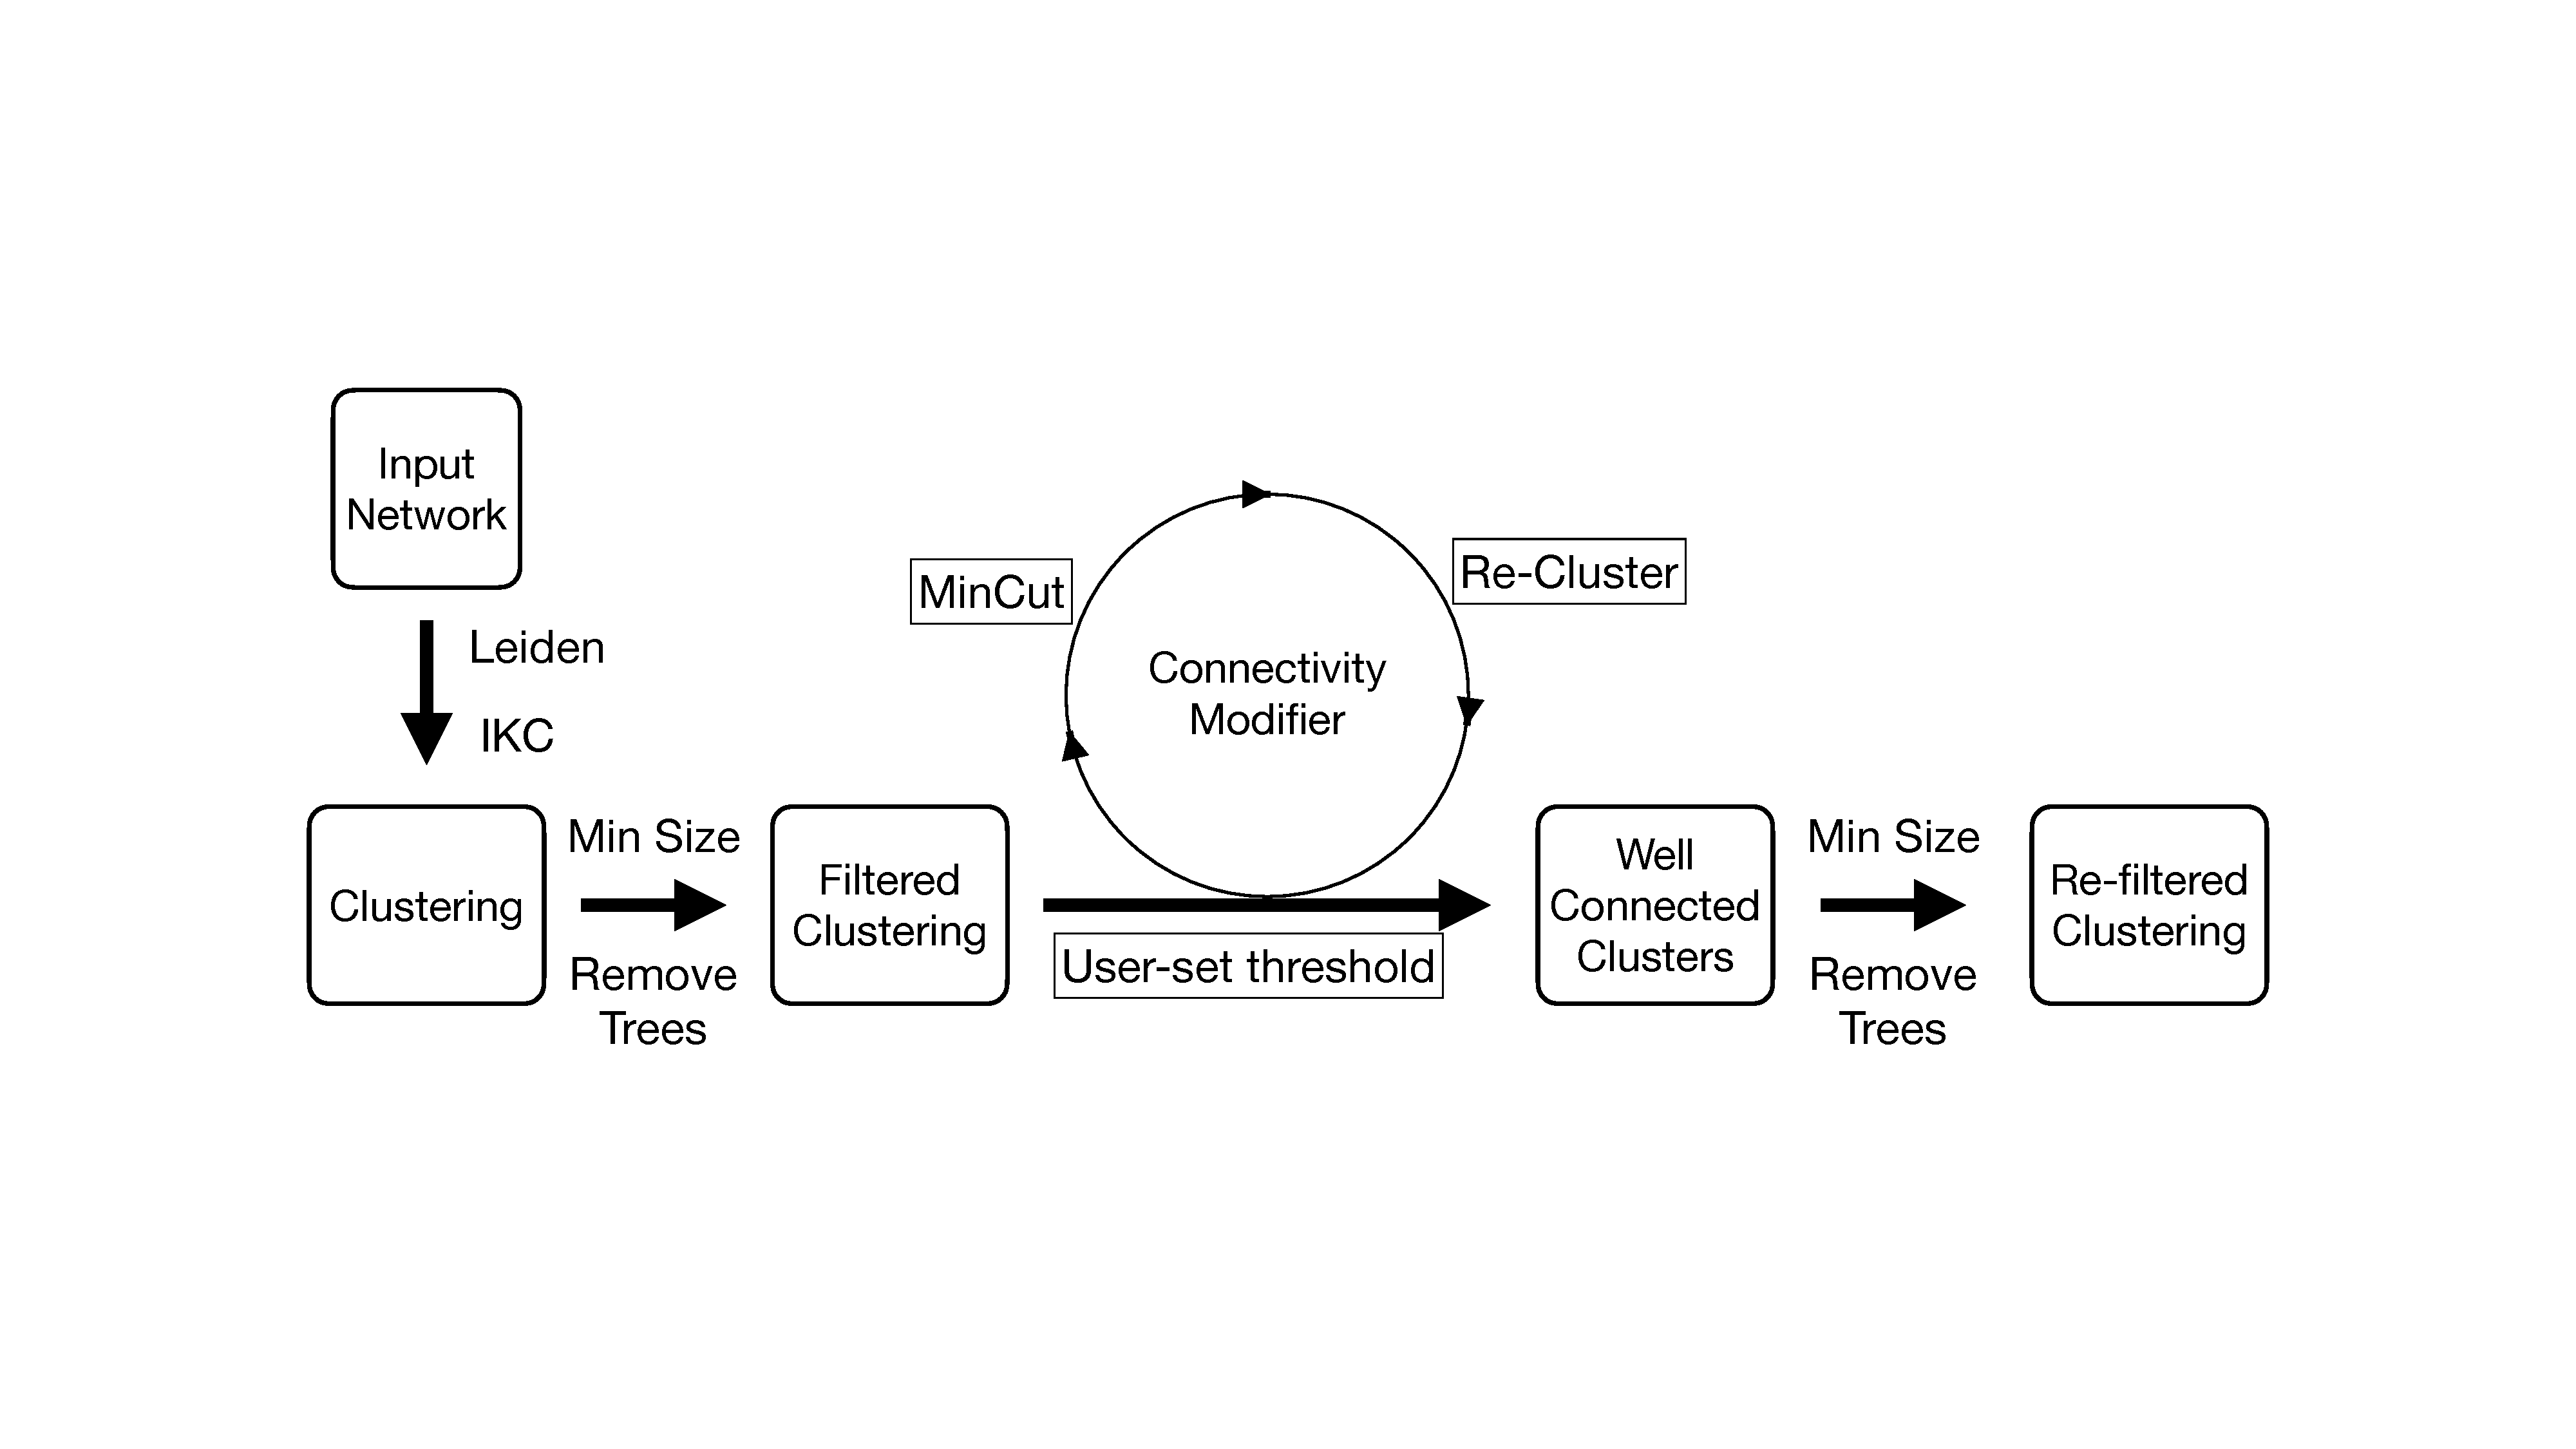
\includegraphics[width=0.7\linewidth]{workflow.pdf}
\caption{Pipeline Schematic.}
\end{figure}

The three clustering methods we enabled are (i) Leiden algorithm optimizing its default quality function, the Constant Potts Model (CPM) (ii) IKC, and (iii) Leiden optimizing modularity. In this study, we report data only from the first two. 
For  a cluster $C$ to be considered``well-connected", we require that the size of the minimum edge cut for $C$ be greater than $\log_{10}(||C||)$ (where $||C||$ denotes the number of vertices in $C$), but this is a parameter that can be modified by the user.  In this study, we also set the minimum cluster size to be 11. 



\subsubsection{Filters} Clusters were filtered to remove trees and any cluster of size $<=$10 using any of a custom R script, sequential or parallelized Python scripts using the Networkit library \citep{Staudt2016}, or Belinda, a Python package [cite supplementary information and insert Github reference to https://github.com/illinois-or-research-analytics/belinda] for clustering analysis.

\subsubsection{Connectivity Modifier} To recursively compute and apply minimum cuts to individual clusters, we used the Connectivity Modifier (CM) code at [insert Github reference to Connectivity Modifier], which uses Viecut \citep{Henzinger2018,Henzinger2019} as a dependency, and takes as input a clustering from either the Leiden algorithm or IKC, and returns a set of clusters that is guaranteed to be
well-connected. 
We filtered the input clustering as above before passing it as input to Connectivity Modifier. [insert references https://pypi.org/project/connectivity-modifier/].

Here we describe the CM code when passed an input  Leiden clustering $\mathcal{C}$  with resolution parameter $r$; modifying this description to work with 
Leiden for modularity or IKC is then straightforward.
CM used with Leiden and parameter $r$ has the following structure.


First, the set $Bin$ is initialized to the empty set  ($\emptyset$).
CM  then orders the clusters in the input clustering into a queue,  marks them as ``clustered", and processes each cluster in the queue in turn.
Given a cluster $C$ in the queue, if it is marked as ``clustered" then CM uses VieCut to find a small cut in $C$;  if the cut is at most $\log_{10}(||C||)$ (where $||C||$ denotes the number of 
vertices in the cluster), then it removes the cut from the network, splitting the cluster $C$ into two  subsets $A$ and $B$.
Both $A$ and $B$ are then added into  queue for subsequent processing, and marked as ``new". 
If the cut size for $C$ was above $\log_{10}(||C||)$, then $C$ is added to $Bin$.
Given a cluster $C$ in the queue that is marked as ``new", it uses Leiden with resolution parameter $r$ on the cluster, thus reclustering $C$
and potentially breaking it up into many subsets; each of these subsets is then added to the queue and marked as ``clustered".
When the queue is empty, the clusters in $Bin$ are returned as the output.

\begin{figure}[H]
\centering
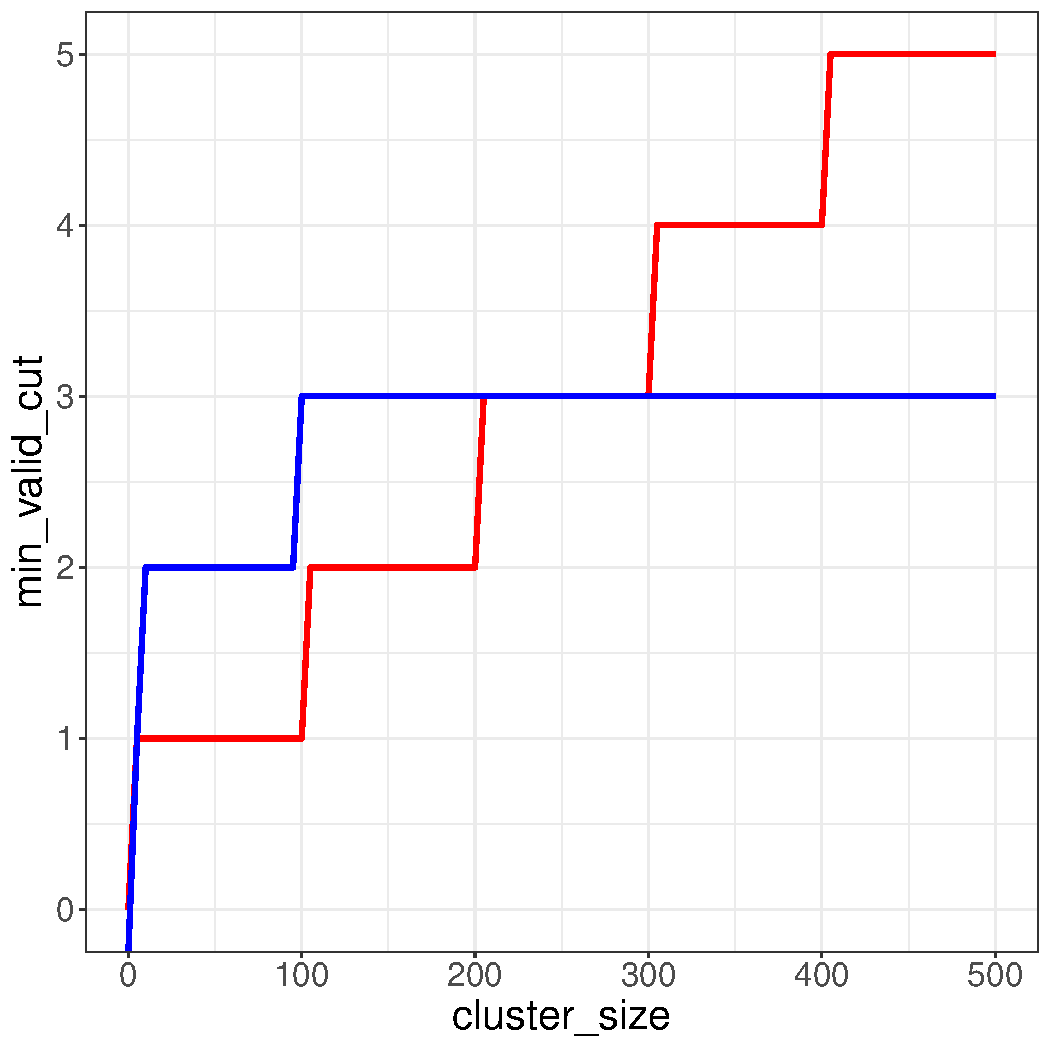
\includegraphics[width=0.7\linewidth]{tandys_figure_3.pdf}
\caption{Tandy's Figure: ceiling(0.01*(x-1)) v  floor(1 + log10(x))}
\end{figure}

The three clustering methods we enabled are (i) Leiden algorithm optimizing its default quality function, the Constant Potts Model (CPM) (ii) IKC, and (iii) Leiden optimizing modularity. In this study, we report data only from the first two. 
For  a cluster $C$ to be considered``well-connected", we require that the size of the minimum edge cut for $C$ be greater than $\log_{10}(||C||)$ (where $||C||$ denotes the number of vertices in $C$), but this is a parameter that can be modified by the user.  In this study, we also set the minimum cluster size to be 11. 


Note that the structure of the CM algorithm ensures that every cluster $C$ in the output is well-connected, since it is 
placed in $Bin$ only if the cut found by VieCut is above $\log_{10}(||C||)$.
However, the CM code as described does not enforce a size constraint.

\textcolor{blue}{For Minhyuk: provide latex for pseudo-code that we can put in the supplement. Make sure it reflects how the algorithm is implemented. On the other hand, and very importantly, the README for the github site says the CM code is a DFS, so this uses a stack and not a queue.  If this is in fact how the algorithm is implemented, then what I wrote is wrong. This needs clarification.} \textcolor{red}{Needs rewrite}.

\subsection{The CM pipeline} \textcolor{blue}{I'm sensing some redundancy between the text above and this section.}
The entire CM pipeline operates in three stages, taking as input (a) the network $N$,  (b) a clustering method with required parameter values,  resolution value for Leiden with CPM ,and $k$ for IKC,
(c)  the initial clustering $\mathcal{C}$ of $N$ using the selected clustering method, 
(d) the required minimum size $B$ for the output clusters ($B=11$ in this study)
and (e) the bound on the minimum cut size as a function of the number of vertices in the cluster $C$
(default $\log_{10}(||C||))$).

\begin{itemize}
\item Stage 1: We perform the filtering, which removes all clusters that are trees or that are below size $B$ from $\mathcal{C}$
\item Stage 2: We run CM on the remaining clusters, returning a set of clusters that are all well-connected
\item Stage 3: We remove resultant clusters that are below size $B$ 
\end{itemize}


\subsection{Data} Several networks were used for testing and analysis and were selected to provide a range of origin, size and edge density. In all cases, below the counts of nodes and edges are reported after removing duplicate records, 
self-citations, and parallel edges from the source data. 

\paragraph{Curated Exosome Network (CEN)}
The CEN is a citation network focused on the exosome research literature consisting of 13,989,436 nodes and 92,051,051 edges. Its construction has previously been previously described in \cite{Jakatdar_2022}.  

\paragraph{Open Citations}
A custom-implemented ETL process was designed to process the publicly available OpenCitations dataset \citep{Peroni2020} and load it into a PostgreSQL table. Citation data was downloaded in Aug 2022. A custom ETL script, written in Bash and SQL, was used to find and pipe uncompressed CSV files, in 20 parallel jobs using the GNU Parallel command-line utility, to a custom function which loaded individual CSV files into a staging view. DOIs were also checked for case differences to remove duplicates.  The resultant network contained 75,025,194 nodes and 1,363,605,603 edges.  [INSERT SECTION ON non-sample based analysis].

\paragraph{SNAP Networks}The following networks were downloaded from the Stanford Network Analysis Project (SNAP) website: (i) cit\_patents \citep{Leskovec2005}, a citation network among US patents (ii) orkut \citep{Yang2013}, data from the Orkut online social network (iii) cit\_hepph \citep{Leskovec2005}, the Arxiv High Energy Physics paper citation network  (iv) wiki\_talk \citep{Leskovec2010}, a network containing users and discussion from the inception of Wikipedia till January 2008 (v) wiki\_topcats \citep{Yin2017}, a web graph of Wikimedia hyperlinks Each network was processed to remove duplicate edges, parallel edges, and self-loops, the numbers of nodes and edges reported below reflect this processing. 

\begin{table}[ht]
\centering
\begin{tabular}{rlllr}
  \hline
 & network & edges & nodes & avg\_deg \\ 
  \hline
  1 & cit\_hepph & 420,877 & 34,546 & 24.37 \\ 
  2 & cit\_patents & 16,518,947 & 3,774,768 & 8.75 \\ 
  3 & orkut & 117,185,083 & 3,072,441 & 76.28 \\ 
  4 & wiki\_talk & 4,659,565 & 2,394,385 & 3.89 \\ 
  5 & wiki\_topcats & 25,444,207 & 1,791,489 & 28.41 \\ 
   \hline
\end{tabular}
% Counts manually verified on Jan 31. 2023 by gc
\caption{Network statistics for cleaned versions of 5 networks downloaded from SNAP and used as benchmarks}
\end{table}

\paragraph{LFR (random) networks}
As a comparison group, synthetic networks were generated using the LFR `benchmark' methodology \citep{Lancichinetti2008}. [Ask Yasamin to write this section up].

\textcolor{blue}{
To do (for Yasamin):}

\begin{itemize}
\item For  the CEN and  for the Open Citations networks, produce one LFR network  that has a mixing parameter and other
parameters set so as to produce something that resembles the given Leiden clustering of the given real-world network. (However, keep the LFR network
on the moderate size, so at most 3,000,000 vertices.)
\textcolor{blue}{This requires that George specify the Leiden clustering for these two networks.}  \textcolor{red}{per discussion on Feb 1, $<=$ 5,000,000 nodes was agreed on).}
\item 
For each LFR network: 
\begin{itemize}
\item Report empirical statistics of the network
\item Report empirical statistics of the true clustering 
\item capture accuracy relative to `ground' truth
\item 
Recluster using Leiden (same resolution value) and then run the CM pipeline.
Record all the usual statistics
\item Run CM on the true clustering.
Report all the usual statistics
\end{itemize}
\end{itemize}

\noindent
The usual statistics are things like:
\begin{itemize}
\item Statistics before running the CM pipeline, including distribution of cluster sizes, node and edge coverage 
\item Statistics at each stage of the CM pipeline (percentage of clusters that are deleted due to being trees,
then deleted due to being too small, then the percentage of remaining clusters  that have small edge cuts).
But at the end of the pipeline we also remove small clusters.  
Also show total node and edge coverage at the end of each stage of the CM pipeline. 
\item 
In essence we want to know which clusters in the input survive the entire process, which ones are modified. 
We'll want their sizes as well, so we can say things like ``20\% of the input clusters above size 100 have small edge cuts" and
``10\% of the input clusters above size 50 are trees".
\end{itemize}

\section{Results and Discussion}

\subsection{Well connected communities from Leiden and IKC clustering.}

We first evaluated a citation network, the CEN (Materials and Methods) consisting of 13,989,436 nodes and 92,051,051 edges, which captures the relatively recent literature relevant to exosomes and extracellular vesicles. We clustered the CEN using Leiden optimizing CPM with resolution values ranging from 0.5 to 0.001 (Table 1). This range of resolution values brackets the resolution values used by us in earlier studies \citep{Wedell2022,Jakatdar_2022}. 

% latex table generated in R 4.1.3 by xtable 1.8-4 package
% Mon Jan 30 22:29:28 2023
% generated by singleton corrected script.
\begin{table}[ht]
\centering
\begin{tabular}{rlrrrrrrr}
  \hline
 & clustering & n=1 & n$>$1 & n$>$10 & min & med & max & node\_cov \\ 
  \hline
1 & leiden 0.5 & 12,701,653 & 433,557 & 8,503 & 11 & 14 & 68 & 0.97 \\ 
  2 & leiden 0.1 & 8,341,818 & 516,299 & 273,420 & 11 & 11 & 319 & 23.98 \\ 
  3 & leiden 0.01 & 3,245,556 & 280,518 & 275,641 & 11 & 28 & 3,186 & 76.52 \\ 
  4 & leiden 0.001 & 2,172,927 & 66,326 & 65,771 & 11 & 98 & 16,481 & 84.45 \\ 
   \hline
\end{tabular}
\caption{Clustering the Curated Exosome Network (CEN) with Leiden. Node coverage and cluster size increase as resolution values is decreased. The first column (clustering) shows the resolution value passed as a parameter to Leiden. The next three columns show cluster counts for singleton clusters, non-singleton clusters, and clusters of size $>10$. Minimum, median, and max cluster sizes are shown for clusters of size $>10$. The last column indicates node coverage expressed as a percentage; the count of nodes in clusters of size $>10$ relative to the total number of nodes in the network. }
\label{tab: table1}
\end{table}

Predictably, node coverage increased as resolution values was decreased. Of interest, however, was whether trees, which are excellent examples of poorly connected clusters, were being generated. Accordingly, we searched for trees in clusterings generated by either Leiden or IKC. In both cases, we filtered out clusters of size $10$ or less before evaluating clusters for the presence of trees. Strikingly, we observed trees in Leiden clusterings from resolution values of 0.1, 0.01, and 0.001 but not a 0.5. At resolution value of 0.1, 273,420 clusters were generated of which 254,734 (93.2\%) were trees of size 11. At a resolution value of 0.001, 65,771 clusters were generated were found of which 22,750 (34.6\%) were trees (Figure 1 and Table 2). Interestingly, as resolution values were decreased further, the number of trees decreased but the average tree size increased (Figure 1, Table 3). 

\begin{figure}[H]
\centering
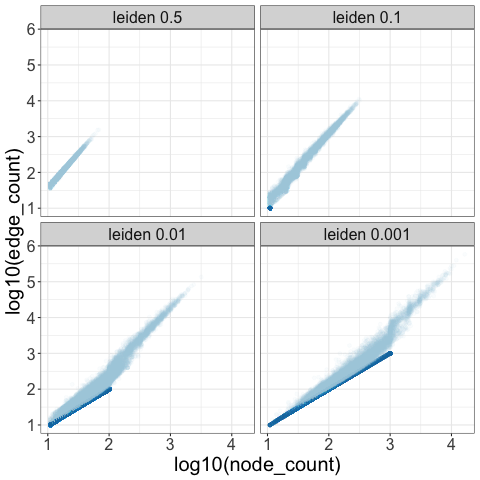
\includegraphics[width=0.7\linewidth]{cen_quad_fig1.png}
\caption{The Curated Exosome Network (CEN) consists of 13,989,436 nodes and 92,051,051 edges. The average degree of its nodes is 13.16. The CEN was clustered at four resolution values (0.5, 0.1, 0.01, 0.001) using the Leiden algorithm with Constant Potts Model as quality function. The figure shows the count of edges in each cluster of size $>$  10 plotted against the count of nodes in each cluster (cluster size). As resolution value decreases, node coverage (the fraction of nodes that are found in clusters of size $>$  10) increases. The number of such clusters does not, however, monotonically increase (Table 1). As the resolution value decreases, tree clusters (dark blue) are detected, with tree size inversely related to resolution value. However, the number of trees decreases as the resolution factor is decreased with the exception of clustering at 0.5 for which no trees are detected. (Table 2).}
\end{figure}

To follow up on the presence of sparse clusters in the form of trees, Leiden clusters were filtered to exclude clusters of size $<=$ 10, after which the number of clusters that were \emph{trees} (the case where \emph{n}, the number of nodes in a cluster, is greater by one than \emph{m}, the number of intra-cluster edges) were counted. Trees were then filtered, after which the remaining clusters were processed with connectivity modifier (CM) using log10(n) as threshold, then filtered again to remove small clusters (Table 2).

% latex table generated in R 4.1.3 by xtable 1.8-4 package
% Sun Jan 29 23:08:57 2023
% generated by running table2.R on odesa in
% /data1/snap_leiden_venv/cen

\begin{table}[ht]
\centering
\begin{tabular}{rllrrrrr}
  \hline
 & clustering & rx & cluster\_count & min & median & max & node\_cov \\ 
  \hline
1 & leiden.5 & -  & 8503 &  11 & 14.00 &  68 & 0.97 \\ 
  2 & leiden.5 & filter & 8503 &  11 & 14.00 &  68 & 0.97 \\ 
  3 & leiden.5 & cm & 8503 &  11 & 14.00 &  68 & 0.97 \\ 
  4 & leiden.5 & filter & 8503 &  11 & 14.00 &  68 & 0.97 \\ 
  5 & leiden.1 & - & 273420 &  11 & 11.00 & 319 & 23.98 \\ 
  6 & leiden.1 & filter & 18686 &  11 & 20.00 & 319 & 3.95 \\ 
  7 & leiden.1 & cm & 14681 &  11 & 20.00 & 319 & 3.63 \\ 
  8 & leiden.1 & filter & 14681 &  11 & 20.00 & 319 & 3.63 \\ 
  9 & leiden.01 & -& 275641 &  11 & 28.00 & 3186 & 76.52 \\ 
  10 & leiden.01 & filter & 64320 &  11 & 34.00 & 3186 & 24.80 \\ 
  11 & leiden.01 & cm & 34071 &  11 & 24.00 & 3186 & 13.20 \\ 
  12 & leiden.01 & filter & 34071 &  11 & 24.00 & 3186 & 13.20 \\ 
  13 & leiden.001 & - & 65771 &  11 & 98.00 & 16481 & 84.45 \\ 
  14 & leiden.001 & filter & 43021 &  12 & 112.00 & 16481 & 62.31 \\ 
  15 & leiden.001 & cm & 27581 &  11 & 32.00 & 16480 & 23.15 \\ 
  16 & leiden.001 & filter & 27581 &  11 & 32.00 & 16480 & 23.15 \\ 
   \hline
\end{tabular}
\caption{Identifying well connected clusters from Leiden clustering of the CEN. For each of resolution values \{0.5, 0.1, 0.01, 0.001\}, clusters were limited to those of size 11 or greater, then depleted of trees, the processed by CM, and then filtered to remove any clusters of size 10 or less as well as trees. Node coverage is least 0.5 and maximum at 0.01 (Table 1). However, removal of trees and CM treatment reduces node coverage by 20.4\%, 63.3\%, and 61.3\% of the original values for resolution values of 0.01, 0.01, and 0.001 respectively.  For example, at resolution value 0.001, node coverage drops from 84.45\% to 23.15\%. At a resolution value of 0.5, no change is observed.}
\label{tab:table2}
\end{table}


% latex table generated in R 4.2.2 by xtable 1.8-4 package
% Sun Jan 15 17:37:03 2023
\begin{table}[ht]
\centering
\begin{tabular}{lrllrrr}
  \hline
 Clustering & Resolution & type & min & med & max \\ 
  \hline
leiden & 0.5 & non\_tree &  11 & 14 &  68 \\ 
leiden & 0.5 & tree &  NA & NA &  NA \\ 
leiden & 0.1 & tree &  11 & 11 &  11 \\ 
leiden  & 0.1 & non\_tree &  11 & 20 & 319 \\ 
leiden  & 0.01 & tree &  11 & 27 & 101 \\ 
leiden & 0.01 & non\_tree &  11 & 34 & 3186 \\ 
leiden & 0.001 & tree &  11 & 65 & 1001 \\ 
leiden & 0.001 & non\_tree &  12 & 112 & 16481 \\ 

   \hline
\end{tabular}
\caption{Cluster sizes for Leiden clusters on the CEN. We show empirical statistics (minimum, median, and maximum) of Leiden clusters generated using the Constant Potts Model (CPM) as quality function and with different resolution values. Clusters of of size at most 10 have been removed. Do we need this table?}
\end{table}

% latex table generated in R 4.2.2 by xtable 1.8-4 package
% Fri Jan 13 18:03:02 2023
\begin{table}[ht]
\centering
\begin{tabular}{lrrrrrr}
  \hline
 clustering & res\_value & clus\_count & node\_cov & min & med & max \\ 
  \hline
Leiden & 0.5 & 297038 & 5.98 &  11 & 13.00 & 183 \\ 
Leiden & 0.1 & 1313856 & 43.78 &  11 & 17.00 & 882 \\ 
Leiden & 0.01 & 1361168 & 88.93 &  11 & 19.00 & 3530 \\ 
Leiden & 0.01 & 232288 & 90.56 &  11 & 64.00 & 23470 \\ 
Leiden & 0.0005 & 133147 & 90.97 &  11 & 90.00 & 39049 \\  
Leiden & 0.0001 & 39069 & 91.81 &  11 & 177.00 & 176557 \\ 
   \hline
\end{tabular}
\caption{Clustering the Open Citations Network. The open citations network (Materials and Methods) consisting of 75,025,194 nodes and 1,363,605,603 edges was clustered with the Leiden algorithm, using the Constant Potts Model (CPM) as quality function, and using various resolution values (column 1). Node coverage is expressed as the the percent of nodes in these clusters of size $>$ 10 relative to the total number of nodes in the network. Minimum, median, and max cluster sizes are shown in the last three columns.  }
\end{table}

\textcolor{blue}{Insert Minhyuk's IKC data for CEN}.


		
\section{Conclusions}
	
\section*{Competing Interests} \vspace{3mm} The authors have no competing interests. 
	
\section*{Funding Information} 
	
\section*{Data Availability} 
	
\section*{Acknowledgments} 

\bibliographystyle{apalike}
\bibliography{cmv1}
\end{document}

% latex table generated in R 4.1.3 by xtable 1.8-4 package
% Sun Jan 22 19:56:56 2023
\begin{table}[ht]
\centering
\resizebox{.5\textwidth}{!}{
\begin{tabular}{rrrrrll}
  \hline
 & clus\_count & min & med & max & type & gp \\ 
  \hline
1 & 20648920 &   2 &   2 &  10 & size 2-10 & leiden.5 \\ 
  2 & 297038 &  11 &  13 & 183 & size $>$10 & leiden.5 \\ 
  3 & 297038 &  11 &  13 & 183 & non\_tree & leiden.5 \\ 
  4 & 10349 &  11 &  13 &  85 & pre-cm & leiden.5 \\ 
  5 & 10349 &  11 &  13 &  85 & post-cm & leiden.5 \\ 
  \hline
  6 & 7324830 &   2 &   5 &  10 & size 2-10 & leiden.1 \\ 
  7 & 1313856 &  11 &  17 & 882 & size $>$10 & leiden.1 \\ 
  8 & 1299838 &  11 &  17 & 882 & non\_tree & leiden.1 \\ 
  9 & 14016 &  11 &  11 &  11 & star & leiden.1 \\ 
  10 &   2 &  11 &  11 &  11 & tree & leiden.1 \\ 
  11 & 45252 &  11 &  15 & 306 & pre-cm & leiden.1 \\ 
  12 & 39954 &  11 &  16 & 306 & post-cm & leiden.1 \\ 
  \hline
  13 & 772769 &   2 &   2 &  10 &  size 2-10 & leiden.01 \\ 
  14 & 1361168 &  11 &  19 & 3530 & size $>$10 & leiden.01 \\ 
  15 & 1034558 &  11 &  24 & 3530 & non\_tree & leiden.01 \\ 
  16 & 8669 &  11 &  18 & 101 & star & leiden.01 \\ 
  17 & 317941 &  11 &  15 &  58 & tree & leiden.01 \\ 
  18 & 36171 &  11 &  21 & 1561 & pre-cm & leiden.01 \\ 
  19 & 29793 &  11 &  16 & 1561 & post-cm & leiden.01 \\ 
  \hline
  20 & 606966 &   2 &   2 &  10 & size 2-10 & leiden.001 \\ 
  21 & 232288 &  11 &  64 & 23470 & size $>$10  & leiden.001 \\ 
  22 & 208543 &  11 &  73 & 23470 & non\_tree & leiden.001 \\ 
  23 & 1476 &  11 &  15 & 1001 & star & leiden.001 \\ 
  24 & 22269 &  11 &  43 & 500 & tree & leiden.001 \\ 
  25 & 7299 &  11 &  63 & 12707 & pre-cm & leiden.001 \\ 
  26 & 11766 &  11 &  43 & 12707 & post-cm & leiden.001 \\ 
  \hline
  27 & 522696 &   2 &   2 &  10 & size 2-10 & leiden.0001 \\ 
  28 & 39069 &  11 & 177 & 176557 & size $>$10 & leiden.0001 \\ 
  29 & 34031 &  11 & 206 & 176557 & non\_tree & leiden.0001 \\ 
  30 & 3525 &  11 &  14 & 267 & tree & leiden.0001 \\ 
  31 & 1513 &  11 &  14 & 251 & star & leiden.0001 \\ 
  32 & 1192 &  11 & 172 & 53195 & pre-cm & leiden.0001 \\ 
  33 & 1971 &  11 & 118 & 51053 & post-cm & leiden.0001 \\ 
   \hline
\end{tabular}}
\caption{test- data being revised to use larger samples}
\end{table}


\paragraph{SNAP benchmarks}
In addition, five more real world networks from the Stanford Network Analysis Project (SNAP) collection \citep{leskovec2016snap} were downloaded in Dec 2022:
\begin{itemize}
\item  \emph{cit\_patents} (3,774,768 nodes, 16,518,947 edges), \
\item \emph{cit\_hepph} (34,546 nodes, 420,877 edges),
\item  \emph{wiki\_topcats} (1,791,489 nodes, 25,444,207 edges)
\item  \emph{orkut} (3,072,441 nodes, 117,185,083 edges). 
\item \emph{wiki\_talk} (2,394,385 nodes, 4,659,565 edges)
\end{itemize}



